\section{Architecture}


Although Ethereum clients with different implementations can agnostically
participate in the system, there is no common agreement on the Ethereum
architecture. Since "an implementation is not an architecture"
\cite{bib:art-of-scalability}, we propose a conceptual model which is inspired
by the OSI reference model. The model is comprised of 5 horizontal layers and 1
vertical layer: the
\begin{enumerate*}[label=(\arabic*)]
  \item network layer, the specification of the network topology, the
  \item propagation layer, how the nodes communicate and which protocols
  are used, the
  \item data layer, the data structures and data types, the
  \item consensus layer, how the nodes reach consensus on the state which is
  represented in the data layer, hence the mining and the transactions execution
  process, and the
  \item application layer, the smart contract as the business logic of the
  system
\end{enumerate*}.

We define the Ethereum Virtual Machine (EVM) as a vertical layer because it
appears in the data, consensus and application layers.

\begin{figure}[H]
	\begin{center}
		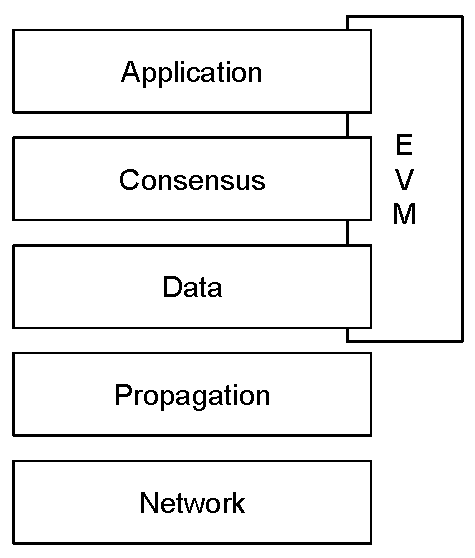
\includegraphics[width=0.4\textwidth]{./res/img/architecture.pdf}
	\end{center}
	\caption{Layers of the Ethereum architecture}
	\label{fig:architecture}
\end{figure}

Since sometime the architecture and the implementation mix up, we could refer to
some implementation details along the description of the layers.






% Describing the Ethereum architecture, first we want to underly the component it
% is comprised of, and subsequently we want to outline the relations between them
% from a functional point of view.

% Ethereum is a peer-to-peer architecture, a decentralized architecture in which
% the nodes are logically equivalent and function as a \emph{servent} (i.e. a that
% node acts as a client and a sever at the same time). In this type of
% architecture, the nodes are formed by processes and the links represent the
% possible communication channels, that is, an \emph{overlay network}
% \cite{van2017distributed} which is discussed in \autoref{sec:overlay-network}.
% The peer-to-peer architectures support the \emph{horizontal distribution} for
% which each node operate on its own share of the complete data set, thus
% balancing the load. Ethereum implement it differently, each node read and write
% its own copy of the complete data set indeed, but rather to achieve consensus of
% the state instead of balancing the load.

% The main components that form Ethereum are:

% \begin{itemize}
%   \item the accounts which, with their address and state, constitute the \textbf{state}
%   \item the \textbf{messages} and the \textbf{transactions}, the main
%   communication channels in Ethereum
%   \item the \textbf{blocks} which, linked together, structure the blockchain
% \end{itemize}


